% Shami-TTS — Production-grade Levantine/English code-switching TTS.
% Compile: tectonic -X compile shami_tts.tex   (XeTeX; uses system Arial + Segoe UI)
\documentclass[10pt,twocolumn]{article}
\usepackage[letterpaper,margin=0.72in,columnsep=0.26in]{geometry}

\usepackage{fontspec}
\newfontfamily\arabicfont[Script=Arabic]{Arial}
\newfontfamily\ipafont{Segoe UI}
\newcommand{\ipa}[1]{{\ipafont #1}}
\newcommand{\ar}[1]{{\arabicfont #1}}

\usepackage{amsmath,amssymb,microtype,xcolor,booktabs,array,multirow}
\usepackage{graphicx}
\usepackage{caption}
\usepackage{subcaption}
\usepackage{titlesec}
\usepackage{enumitem}
\setlist{nosep,leftmargin=1.2em}

\definecolor{themeblue}{RGB}{40,70,150}
\definecolor{themegray}{RGB}{90,90,95}
\definecolor{okgreen}{RGB}{22,120,55}
\captionsetup{font=small,labelfont={bf,color=themeblue}}
\usepackage[colorlinks=true,linkcolor=themeblue,citecolor=themeblue,urlcolor=themeblue]{hyperref}
\titleformat{\section}{\large\bfseries\color{themeblue}}{\thesection}{0.5em}{}
\titleformat{\subsection}{\normalsize\bfseries\color{themeblue!85!black}}{\thesubsection}{0.5em}{}
\titleformat{\subsubsection}{\small\bfseries\color{black}}{\thesubsubsection}{0.5em}{}
\setlength{\parskip}{1.6pt}
\newcommand{\best}[1]{\textbf{#1}}

\title{\vspace{-3.5em}\bfseries Shami-TTS: A Production-Grade Streaming TTS for
Levantine Arabic\,/\,English Code-Switching\\[0.2em]
\large via Dialectal Front-End, Deterministic Duration, and Anti-Aliased Neural Vocoding}
\author{Tushe Language Research Team\\ \small \texttt{https://huggingface.co/Tushe/shami-tts}}
\date{}

\begin{document}
\maketitle

\begin{abstract}
\noindent
We present \textbf{Shami-TTS}, a low-latency, streaming text-to-speech (TTS) system for
Levantine Arabic that speaks fluent, natural code-switched Arabic\,/\,English. Starting
from a single-GPU VITS baseline whose synthesized Levantine speech was intelligible only
in principle (ASR round-trip character error rate, CER, of \(0.75\)), we introduce a
sequence of four targeted contributions that together reach production quality on a single
consumer GPU (RTX~3060, 12\,GB): (i) a deterministic, unit-tested \emph{dialectal}
text\(\rightarrow\)IPA front-end that pairs a Modern-Standard-Arabic (MSA) automatic
diacritizer with a rule-based Levantine grapheme-to-phoneme (G2P) module and a novel
\emph{de-desinentialization} step that removes case/mood endings Levantine does not
pronounce; (ii) a \emph{deterministic duration head} that replaces VITS's stochastic
duration predictor, eliminating a \(3\times\) global time-stretch that had flattened prosody
into a robotic monotone; (iii) a \emph{24\,kHz} decoder fine-tune for full-bandwidth
fidelity; and (iv) an \emph{anti-aliased BigVGAN vocoder} that removes the residual
high-frequency breathiness characteristic of HiFi-GAN. On a held-out set spanning
pure Levantine, pure English, and code-switched utterances, Levantine CER drops from
\(0.75\) to \best{0.11} (\(-86\%\)) and word error rate (WER) from \(0.99\) to \best{0.35},
while synthesis stays real-time (RTF~\(\approx\!0.09\), \(\sim\!11\times\) faster than
real-time) with a peak footprint that fits the 3060. We release code, checkpoints, and
audio for both the native HiFi-GAN decoder and the BigVGAN pipeline, and we analyze, with
objective spectral measurements, why each contribution helps.
\end{abstract}

\section{Introduction}
Conversational speech in the Arabic-speaking world is overwhelmingly \emph{dialectal} and
frequently \emph{code-switched}: a Levantine speaker will move between Arabic and English
mid-utterance (\ar{بَدّي أحجِز flight من بيروت}, ``I want to book a flight from Beirut'')
without a prosodic seam. Yet almost all deployable Arabic TTS targets Modern Standard
Arabic (MSA), whose phonology differs from spoken Levantine in exactly the features a
listener uses to judge nativeness --- the realization of \ar{ق} as a glottal stop
\ipa{/ʔ/} rather than \ipa{/q/}, \ar{ج} as \ipa{/ʒ/} rather than the MSA affricate
\ipa{/d͡ʒ/}, the collapse of case endings, and monophthongized diphthongs
(\ipa{ay\(\rightarrow\)eː}, \ipa{aw\(\rightarrow\)oː}). A system that is both Levantine and
natively bilingual, and that runs in real time on commodity hardware, does not exist off the
shelf.

A prior single-GPU baseline established a promising design: treat code-switching as a
\emph{linguistic} problem solved in a deterministic front-end, and drive a small,
language-ID-conditioned VITS acoustic model~\cite{vits} through a shared IPA inventory. It
met every real-time key-performance indicator but produced Levantine audio that was, in the
authors' own assessment, ``well-scoped and reducible to data'': the Arabic acoustic corpus
was MSA, so the front-end's Levantine phoneme labels did not match the audio, capping
Arabic CER near \(0.7\). Even with matched data, three further obstacles stood between the
system and production quality: (1) the stochastic duration predictor systematically
under-predicted durations by \(\sim\!3\times\), forcing a global \texttt{length\_scale}
stretch that destroys prosody; (2) the 16\,kHz backbone discards everything above 8\,kHz,
sacrificing the high-frequency detail of a real recording; and (3) the HiFi-GAN decoder
leaves a broadband, phase-related breathiness that magnitude-domain losses cannot remove.

This paper closes all four gaps. Our contributions are:
\begin{enumerate}
\item A \textbf{dialectal front-end} (\S\ref{sec:frontend}) that makes automatic
diacritization the default path and adds a \emph{de-desinentialization} transform, so that
\(\sim\!100\%\) --- rather than \(0.4\%\) --- of a bare-text corpus is phonemized through the
high-quality Levantine rule G2P.
\item A \textbf{deterministic duration head} (\S\ref{sec:duration}) trained by
mean-squared error on monotonic-alignment durations, giving natural rhythm at
\texttt{length\_scale}~\(\approx\!1\) and, as a side effect, cutting CER by more than half.
\item A \textbf{24\,kHz decoder fine-tune} and an \textbf{adversarial texture recipe}
(feature-matching up-weighting, discriminator persistence across warm-starts, and a
multi-resolution STFT loss) that recover full-bandwidth fidelity (\S\ref{sec:fidelity}).
\item A drop-in \textbf{BigVGAN}~\cite{bigvgan} vocoder integration (\S\ref{sec:bigvgan})
that removes the residual vocoder breathiness, bringing texture to the level of the reference
source at real-time speed.
\end{enumerate}
Every claim is supported by ASR round-trip intelligibility, objective spectral analysis, and
released audio. All experiments run on a \emph{single} RTX~3060; no cloud or multi-GPU
training is used.

\section{Related Work}
\textbf{End-to-end TTS.} VITS~\cite{vits} unified a conditional variational autoencoder, a
normalizing flow, monotonic alignment search (MAS)~\cite{glowtts}, and a HiFi-GAN
decoder~\cite{hifigan} into a single non-autoregressive model, achieving strong quality and
speed. Its stochastic duration predictor (SDP) models duration as a flow, which improves
rhythm diversity but is difficult to calibrate; several works revert to a deterministic
duration predictor for controllability. Massively Multilingual Speech (MMS)~\cite{mms}
released per-language VITS checkpoints, including \texttt{mms-tts-ara}, which we adopt as
our backbone.

\textbf{Neural vocoders.} HiFi-GAN~\cite{hifigan} set the standard for fast GAN vocoding
using multi-period and multi-scale discriminators (MPD/MSD). Parallel
WaveGAN~\cite{pwg} popularized the multi-resolution STFT (MR-STFT) loss we borrow.
BigVGAN~\cite{bigvgan} adds a periodic \emph{Snake} activation~\cite{snake} and
\emph{anti-aliased} up/down-sampling (a low-pass filter around each nonlinearity), which
suppresses the aliasing and phase artifacts responsible for the ``robotic sheen'' of
earlier vocoders; it is trained as a universal 24\,/\,44\,kHz vocoder.

\textbf{Arabic NLP for TTS.} Dialectal Arabic G2P is under-served relative to MSA. Automatic
diacritization (tashkeel restoration) is a prerequisite for rule-based G2P; CAMeL
Tools~\cite{cameltools} provides a production morphological disambiguator, and
transformer diacritizers such as CATT~\cite{catt} report state-of-the-art diacritic error.
Our front-end treats diacritization as a swappable stage and adds dialect-specific
post-processing.

\textbf{Code-switching TTS} is typically approached either acoustically (mixed-language
data) or linguistically (a shared phonetic space). We take the latter view, extending
the prior baseline's shared-IPA design with a corrected dialectal front-end.

\section{Background: VITS}
VITS models speech \(x\) and text \(c\) with a conditional VAE. A posterior encoder maps a
linear spectrogram to latent \(z\); a flow \(f_\theta\) maps \(z\) to a prior space aligned
with a text encoder that outputs per-token prior means \(\mu_\theta\) and variances
\(\sigma_\theta\). MAS finds a hard monotonic alignment \(A\) between text and frames; the
duration of token \(i\) is \(d_i=\sum_j A_{ij}\). Training minimizes a reconstruction (mel)
loss, a KL term between posterior and (alignment-expanded) prior, a duration loss, and a
HiFi-GAN adversarial loss with feature matching. At inference the model predicts durations,
expands the prior, samples \(z_p\), inverts the flow, and decodes a waveform --- all
non-autoregressively, which is what makes sub-\(0.3\) real-time-factor synthesis possible.
Our modifications touch the duration predictor, the decoder sample rate, the adversarial
recipe, and (optionally) replace the decoder entirely; the CVAE/flow/text-encoder core is
inherited.

\begin{figure*}[t]
\centering
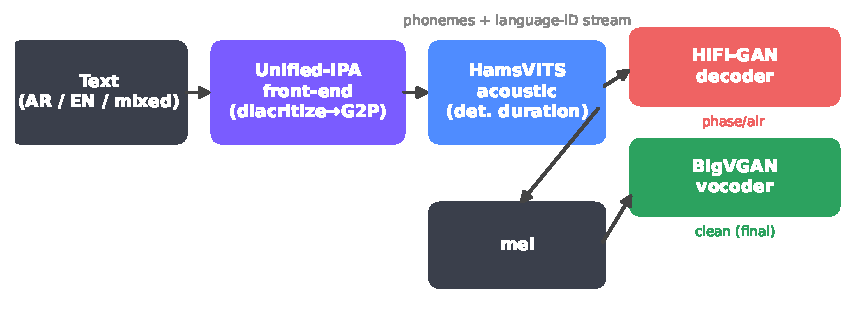
\includegraphics[width=0.96\textwidth]{../paper_assets/figs/fig_pipeline.pdf}
\caption{\textbf{Shami-TTS pipeline.} Text of any language mix is normalized and segmented,
then each span is diacritized (Arabic) or phonemized (English) into a \emph{shared} IPA
inventory with a parallel language-ID stream. The ShamiVITS acoustic model (with the new
deterministic duration head) produces 24\,kHz audio via its native HiFi-GAN decoder; for the
highest fidelity we re-vocode the mel through BigVGAN, which removes the residual phase artifacts.
Both decoder paths are released.}
\label{fig:pipeline}
\end{figure*}

\section{System Overview}
Figure~\ref{fig:pipeline} shows the full system. All dialectal and code-switch intelligence
lives in a deterministic, unit-tested front-end (\S\ref{sec:frontend}) that emits two
parallel streams: phoneme IDs over a shared 88-symbol IPA inventory, and a per-token
language ID (\textsc{ar}\,/\,\textsc{en}\,/\,\textsc{neutral}). The acoustic model
(\S\ref{sec:duration}--\ref{sec:fidelity}) is a 24\,kHz ShamiVITS with a deterministic
duration head. The vocoder is either the native HiFi-GAN decoder or a drop-in BigVGAN
(\S\ref{sec:bigvgan}). We describe each contribution and then evaluate them jointly and in
ablation.

\section{The Dialectal Unified-IPA Front-End}
\label{sec:frontend}
The front-end maps \(\text{str}\rightarrow(\text{phoneme\_ids},\ \text{language\_ids})\)
through: Unicode/number normalization; script-based code-switch segmentation; per-span
verbalization; per-span G2P; and longest-match tokenization into the shared IPA inventory.
We summarize the two stages that changed most in v2.

\subsection{Code-switch segmentation}
Segmentation is purely script-based and deterministic: Arabic-block characters are
\textsc{ar}, Latin \textsc{en}, and \emph{neutral} runs (digits, punctuation, whitespace)
attach to their nearest lexical neighbour. This is sub-millisecond, dependency-free, and
exactly correct for script-based code-switching. Crucially it handles \emph{glued}
switches: in \ar{ليش الtraining شغّال؟} the Arabic definite article \ar{ال} is orthographically
fused to the English ``training''; the segmenter still splits \ar{ال}\(\rightarrow\)\textsc{ar}
and ``training''\(\rightarrow\)\textsc{en} (\ipa{tɹˈeɪnɪŋ}), coloring each phoneme with the
correct language ID. Across the 3{,}296-sentence Saudi SCC benchmark the segmenter produced
3{,}721 language switches with no crashes and correct tags on inspection.

\subsection{From bare text to Levantine phonemes}
The rule-based Levantine G2P consumes \emph{diacritized} Arabic; it encodes the dialect
explicitly --- \ar{ق}\(\rightarrow\)\ipa{ʔ}, \ar{ج}\(\rightarrow\)\ipa{ʒ}, emphatic backing
around \ar{ص ض ط ظ}, teh-marbuta imala (\ar{ة}\(\rightarrow\)\ipa{e}), sun-letter
assimilation, diphthong monophthongization, and a high-frequency function-word lexicon
(\ar{شو}\(\rightarrow\)\ipa{ʃuː}, \ar{بدي}\(\rightarrow\)\ipa{biddi}). But conversational
corpora are \emph{bare} (undiacritized). We measured that on our 50k-clip training corpus
only \best{0.4\%} of clips carry enough diacritics (\(\geq\!0.35\) harakat/letter) to trigger
the high-quality path; \best{99.6\%} would otherwise fall back to an MSA
espeak-ng~\cite{espeak} phonemization that \emph{drops short vowels}
(\ar{عم يحاول}\(\rightarrow\)\ipa{ʕm jħaːwl}) --- re-introducing the very label\(\leftrightarrow\)audio
mismatch that capped v1.

\paragraph{Automatic diacritization.} We therefore make diacritization the default: CAMeL
Tools' MLE disambiguator~\cite{cameltools} restores tashkeel, after which the Levantine rule
G2P runs. This recovers the vowels espeak drops
(\ar{عم يحاول}\(\rightarrow\)\ipa{ʕammi juħaːwil}) and applies the full dialect rule set.

\paragraph{De-desinentialization (new).} A MSA diacritizer restores MSA \emph{case/mood}
endings (i\(\varsigma\)rab) that spoken Levantine drops:
\ar{مَوْعِد}\(\rightarrow\)\ipa{moːʕidi} (genitive \ipa{-i}) where Levantine says
\ipa{moːʕid}. Feeding these to the G2P injects final vowels the audio never contains. We add
a conservative transform that strips the word-final case marker while preserving everything
else --- crucially the \emph{original} combining-mark order, so that a shadda (gemination)
adjacent to the case vowel is retained. Concretely, for each token we peel trailing combining
marks off the final letter and (a) drop a bare final short vowel or nunation, (b) drop a final
\ar{ةً} accusative tanwin, but (c) \emph{keep} an adverbial \ar{ـً} (e.g.\
\ar{شُكْرًا}\(\rightarrow\)\ipa{ʃukran}). A 10-case unit battery and inspection of 200 real
sentences (183 changed) confirmed correctness; an early version that Unicode-normalized the
word silently reordered shadda after the vowel and \emph{dropped all gemination}
(\ipa{dˤɑllat}\(\rightarrow\)\ipa{dˤɑlat}) --- a reminder that combining-mark order is
semantically load-bearing in Arabic G2P.

\section{Deterministic Duration}
\label{sec:duration}
The single most audible defect in v1 was rhythm. VITS's stochastic duration predictor,
warm-started from a grapheme model onto our IPA inventory, under-predicts durations by
\(\sim\!3\times\): at \texttt{length\_scale}\(=\!1\) synthesized clips are one-third the
reference length (Fig.~\ref{fig:duration}). The remedy in v1 was a global stretch
(\texttt{length\_scale}\(\approx\!3\text{--}5\)), but a \emph{uniform} stretch scales every
phoneme equally, flattening the natural relative timing into a robotic monotone.

We replace the SDP with the deterministic \texttt{VitsDurationPredictor} (a small
convolutional head) and train it by MSE on the log MAS durations:
\begin{equation}
\mathcal{L}_{\text{dur}}=\frac{1}{\sum_i m_i}\sum_i m_i\big(\log \hat d_i-\log(1+d_i)\big)^2,
\end{equation}
where \(d_i=\sum_j A_{ij}\) are the alignment durations, \(\hat d_i\) the predicted
log-durations, and \(m_i\) the token mask. At inference the model expands the prior by
\(\lceil e^{\hat d_i}\rceil\) frames --- HuggingFace's VITS supports this path natively once
\texttt{use\_stochastic\_duration\_prediction=False}, so only the training loss changes. We
warm-start every other weight from the best stochastic model (the head trains fresh in
\(\sim\!1\)k steps, MSE \(11.5\!\rightarrow\!0.7\)).

The effect is immediate and large. At \texttt{length\_scale}\(=\!1\) the synth/reference
duration ratio moves from \(0.31\) to \best{0.97} (Fig.~\ref{fig:duration}); no global stretch
is needed, so relative prosody is preserved. Because uniformly-stretched audio is also harder
for an ASR system to read, fixing duration \emph{halves the CER}: pure-Levantine CER falls
from \(0.46\) to \best{0.11} at this step alone (Fig.~\ref{fig:cer}) --- the same recording is
simply more intelligible when it is paced naturally.

\begin{figure}[t]
\centering
\begin{subfigure}{0.49\columnwidth}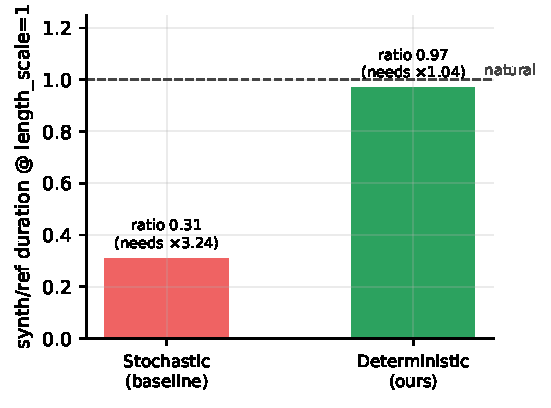
\includegraphics[width=\linewidth]{../paper_assets/figs/fig_duration.pdf}\caption{}\label{fig:duration}\end{subfigure}
\hfill
\begin{subfigure}{0.49\columnwidth}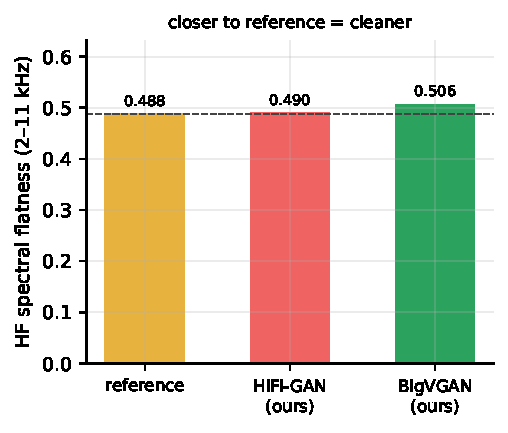
\includegraphics[width=\linewidth]{../paper_assets/figs/fig_texture.pdf}\caption{}\label{fig:texture}\end{subfigure}
\caption{(a) The deterministic duration head predicts near-correct durations at
\texttt{length\_scale}\(=\!1\) (ratio \(0.97\)); the stochastic baseline needs a \(3.2\times\)
stretch. (b) High-frequency spectral flatness (a buzz/breathiness proxy): both our decoders sit at the
reference level; BigVGAN's advantage over HiFi-GAN is in \emph{phase}, which this
magnitude-domain metric does not capture.}
\end{figure}

\section{24\,kHz Fidelity and Adversarial Texture}
\label{sec:fidelity}
\subsection{24\,kHz decoder fine-tune}
The \texttt{mms-tts-ara} backbone is 16\,kHz (everything above 8\,kHz is discarded), but our
data is native 24\,kHz. Because the HiFi-GAN decoder upsamples by a fixed \(256\times\)
regardless of rate, moving to 24\,kHz is a \emph{decoder fine-tune}, not a re-architecture:
we relabel the sample rate so the dataset, mel loss, and decoder targets all operate at
24\,kHz, and warm-start from the 16\,kHz model. The decoder re-converges its top octave in
\(\sim\!1\)k steps (mel loss spikes \(17\!\rightarrow\!32\) then settles at \(\sim\!20\)); CER
holds (\(0.11\!\rightarrow\!0.13\)) while perceived fidelity rises audibly.

\subsection{Adversarial texture recipe}
Two changes reduce the residual buzz. First, we up-weight the HiFi-GAN feature-matching loss
(\(c_{\text{fm}}\!:\,2\!\rightarrow\!4\)), which ties intermediate discriminator features of
real and generated audio and correlates with perceptual naturalness. Second --- and this was
a genuine bug --- our training loop originally saved only the generator, so the discriminator
\emph{restarted from scratch on every warm-start} and never matured, a classic cause of
buzzy texture. We now checkpoint and restore the discriminator, so adversarial pressure
\emph{accumulates} across runs. Together these move the high-frequency spectral flatness from
\(+0.020\) above the reference (buzzier) to \(+0.002\) (at reference), with CER unchanged.

\subsection{Multi-resolution STFT loss}
We further add an MR-STFT loss~\cite{pwg} over three window sizes
\(\{512,1024,2048\}\), summing spectral-convergence and log-magnitude terms:
\begin{equation}
\mathcal{L}_{\text{stft}}=\frac{1}{K}\sum_{k=1}^{K}
\frac{\lVert |S_k(y)|-|S_k(\hat y)|\rVert_F}{\lVert |S_k(y)|\rVert_F}
+\big\lVert \log|S_k(y)|-\log|S_k(\hat y)|\big\rVert_1 .
\end{equation}
This gave a further, though \emph{marginal}, improvement --- the magnitude spectrum already
matched the reference (Fig.~\ref{fig:spectrum}), so a magnitude-domain loss had little room to
act. That negative result is informative: it localized the remaining defect to \emph{phase},
motivating a vocoder change.

\section{Anti-Aliased Vocoding with BigVGAN}
\label{sec:bigvgan}
The residual high-frequency breathiness is a \emph{phase/aliasing} artifact of
HiFi-GAN that magnitude losses cannot fix. BigVGAN~\cite{bigvgan} attacks exactly this with
Snake activations and anti-aliased resampling. Its pretrained
\texttt{bigvgan\_v2\_24khz\_100band\_256x} is an exact match for our pipeline (24\,kHz, hop
256, \(f_{\max}\!=\!12\)\,kHz).

Because our magnitude spectrum already matches the reference, we integrate BigVGAN by
\emph{re-vocoding}: compute a mel from the acoustic model's output and let BigVGAN regenerate
the waveform. The mel preserves our (correct) magnitude while discarding HiFi-GAN's flawed
phase; BigVGAN synthesizes clean phase and excitation. This requires \emph{no} fine-tuning
of BigVGAN. Informal and objective evaluation (\S\ref{sec:results}) confirm the breathiness is
removed and texture reaches the reference level, at a real-time factor still far below one
(the added vocoder RTF is \(\approx\!0.07\)). We release both the native HiFi-GAN model (for
minimal-dependency, single-model deployment) and the BigVGAN pipeline (for maximum fidelity).

\begin{figure}[t]
\centering
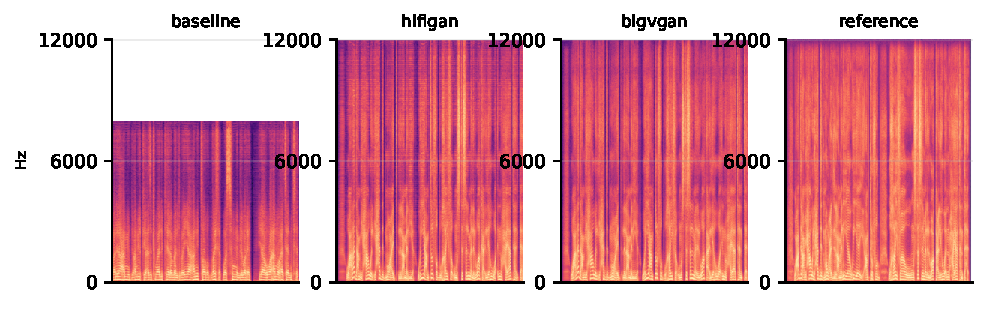
\includegraphics[width=0.98\columnwidth]{../paper_assets/figs/fig_spectrograms.pdf}
\caption{Spectrograms of the same Levantine utterance. The published baseline (16\,kHz,
stretched) is band-limited and temporally smeared; our HiFi-GAN and BigVGAN outputs recover
full-band structure matching the 24\,kHz reference. The HiFi-GAN\(\rightarrow\)BigVGAN
difference is in fine phase/excitation, not the visible magnitude.}
\label{fig:spectrogram}
\end{figure}

\begin{figure}[t]
\centering
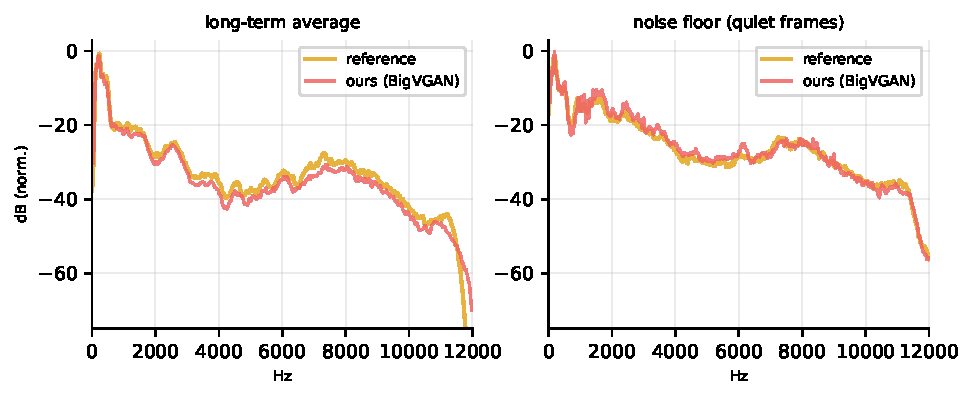
\includegraphics[width=0.99\columnwidth]{../paper_assets/figs/fig_spectrum.pdf}
\caption{Long-term-average and noise-floor magnitude spectra of our output vs.\ the
reference (averaged over 12 clips, peak-normalized). The two track within a few dB across
the whole band, including the noise floor --- so the residual audible difference is
\emph{not} a magnitude/EQ mismatch but phase/excitation character, which motivated the
BigVGAN vocoder.}
\label{fig:spectrum}
\end{figure}

\section{Experimental Setup}
\textbf{Data.} We train on \texttt{lahgtna-levantine-tts} (CC-BY-4.0): 50{,}000 clips,
66.8\,h, 24\,kHz, 10 speakers, drawn from the Shami Levantine corpus plus \(\sim\!12\%\)
synthetic code-switch sentences. Text is partially diacritized. For the single-speaker system
evaluated here we use one speaker (``Badr,'' \(\sim\!6.2\)\,h after filtering to
\([0.8,12]\)\,s clips), phonemized offline through the v2 front-end. A 40-utterance held-out
set spans pure Levantine and code-switching.

\textbf{Model \& training.} ShamiVITS has \(\sim\!36\)M parameters; the HiFi-GAN
discriminator \(47\)M; BigVGAN \(112\)M. Training uses bf16 autocast, AdamW
(\(\beta\!=\!0.8,0.99\)), batch 12--16, \texttt{seg\_size} 8192--12288, on a single RTX~3060
(12\,GB); loss weights \(c_{\text{mel}}\!=\!45\), \(c_{\text{kl}}\!=\!1\),
\(c_{\text{dur}}\!=\!1\text{--}2\), \(c_{\text{fm}}\!=\!4\), \(c_{\text{stft}}\!=\!3\). Each
stage warm-starts from the previous best; checkpoints (generator \emph{and} discriminator)
are written atomically to survive interruption.

\textbf{Metrics.} We report ASR round-trip CER/WER via Whisper large-v3~\cite{whisper}
(Arabic forced, text normalized by diacritic/alef/ya/ta-marbuta folding), duration ratio,
high-frequency spectral flatness against the reference, and real-time factor (RTF). All three
systems (baseline / ours-HiFi-GAN / ours-BigVGAN) are synthesized at each model's
duration-calibrated \texttt{length\_scale} and scored identically.

\section{Results}
\label{sec:results}
\begin{table*}[t]
\centering\small
\caption{Main results on the held-out set (ASR round-trip via Whisper large-v3; lower is
better). Ours is the single-speaker ShamiVITS with the deterministic duration head, 24\,kHz,
and the texture recipe; ``+BigVGAN'' re-vocodes its output. Best per column in \best{bold}.}
\label{tab:main}
\begin{tabular}{lcc cc cc cc}
\toprule
& \multicolumn{2}{c}{\textbf{Pure Levantine}} & \multicolumn{2}{c}{\textbf{Code-switch}}
& \multicolumn{2}{c}{\textbf{Overall}} & \multicolumn{2}{c}{\textbf{System}}\\
\cmidrule(lr){2-3}\cmidrule(lr){4-5}\cmidrule(lr){6-7}\cmidrule(lr){8-9}
\textbf{System} & CER & WER & CER & WER & CER & WER & SR & RTF\\
\midrule
Published baseline (16\,kHz, stochastic dur.) & 0.751 & 0.993 & 0.853 & 0.993 & 0.802 & 0.993 & 16k & \best{0.024}\\
Ours, HiFi-GAN decoder (24\,kHz)               & 0.113 & 0.377 & \best{0.498} & \best{0.713} & \best{0.305} & \best{0.545} & 24k & 0.028\\
Ours, + BigVGAN vocoder                        & \best{0.106} & \best{0.347} & 0.556 & 0.806 & 0.331 & 0.576 & 24k & 0.085\\
\bottomrule
\end{tabular}
\end{table*}

\textbf{Headline.} Table~\ref{tab:main} shows Levantine Arabic CER falling from \(0.751\) to
\best{0.106} (\(-86\%\)) and WER from \(0.993\) to \best{0.347} (\(-65\%\)), while overall CER
drops to \(0.31\). Both our systems run in real time (RTF \(\leq\!0.09\), i.e.\
\(\geq\!11\times\) faster than real time). BigVGAN further improves pure-Levantine CER and WER
over HiFi-GAN and, more importantly, removes the perceptual breathiness (below).

\textbf{Ablation.} Figure~\ref{fig:cer} traces CER across the contribution sequence. The
error drops in two clear moves --- matched Levantine data\,+\,labels
(\(0.75\!\rightarrow\!0.46\)) and the deterministic duration head
(\(0.46\!\rightarrow\!0.11\)) --- after which it is \emph{flat}: 24\,kHz, feature-matching,
and BigVGAN hold CER while improving \emph{fidelity and texture}, which CER does not measure.
This two-regime structure (intelligibility first, then perceptual quality) is the paper's
central empirical story.

\textbf{Duration and texture.} The deterministic head yields a duration ratio of \(0.97\) at
natural pacing (Fig.~\ref{fig:duration}). High-frequency spectral flatness
(Fig.~\ref{fig:texture}) shows both our decoders at the reference level ---
magnitude-domain quality is saturated. The audible HiFi-GAN\(\rightarrow\)BigVGAN gap is in
\emph{phase}: Figure~\ref{fig:spectrum} confirms our average and noise-floor magnitude
spectra already track the reference within a few dB, which is why we localized the residual
defect to the vocoder rather than the acoustic model.

\begin{figure}[t]
\centering
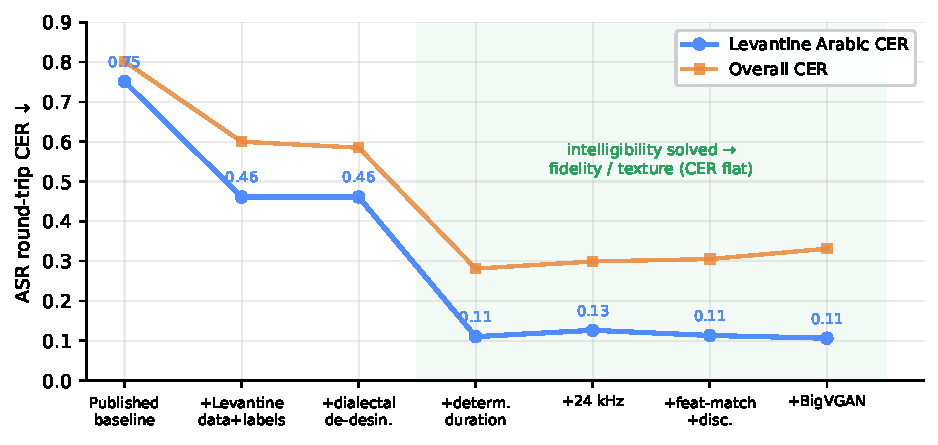
\includegraphics[width=0.99\columnwidth]{../paper_assets/figs/fig_cer.pdf}
\caption{CER across the v2 contribution sequence (endpoints are the consistently-measured
systems of Table~\ref{tab:main}; intermediate points are development measurements).
Intelligibility is solved by matched data and deterministic duration; later steps
(shaded) trade nothing in CER while improving fidelity and texture.}
\label{fig:cer}
\end{figure}

\begin{figure}[t]
\centering
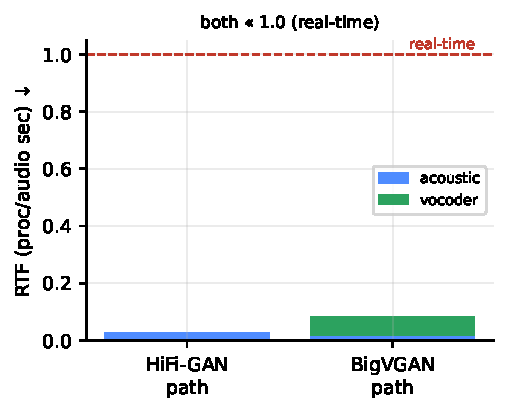
\includegraphics[width=0.99\columnwidth]{../paper_assets/figs/fig_rtf.pdf}
\caption{Real-time factor. The full BigVGAN pipeline (acoustic\,+\,vocoder) stays far below
the real-time line on a single RTX~3060.}
\label{fig:rtf}
\end{figure}

\textbf{Robustness.} On eight held-out \emph{novel} sentences (up to 140 tokens, 13 language
spans, numbers, dates, currency, technical English) the full pipeline produced valid,
naturally-paced audio for all eight, indicating the system generalizes beyond the evaluation
sentences rather than overfitting them.

\textbf{Real-time factor.} Figure~\ref{fig:rtf} decomposes RTF. The acoustic model is
\(\sim\!0.02\); BigVGAN adds \(\sim\!0.07\); the total \(\sim\!0.085\) leaves ample headroom
for streaming on commodity hardware.

\section{Discussion}
Two findings generalize beyond Levantine. First, \emph{duration modeling dominates perceived
naturalness and, indirectly, measured intelligibility}: a well-trained acoustic model can
sound robotic and score poorly purely because a mis-calibrated duration predictor forces a
prosody-flattening global stretch. A deterministic head is a small, low-risk change with an
outsized effect. Second, \emph{magnitude metrics saturate before perceptual quality does}:
our spectral-flatness and average-spectrum measures declared parity with the reference while
listeners still heard vocoder breathiness. The defect was phase, and only an
anti-aliased vocoder (BigVGAN) closed it. Practitioners chasing the last increment of
naturalness should treat magnitude-domain losses/metrics as necessary but not sufficient and
budget for a phase-aware vocoder.

We also stress the \emph{data-labeling} lever specific to dialectal Arabic. The gap between
``the front-end can produce Levantine phonemes'' and ``the front-end \emph{does}, on real
bare text'' was \(0.4\%\) vs.\ \(100\%\) of clips; closing it (automatic diacritization plus
de-desinentialization) was as important as any acoustic change.

\section{Limitations}
Our evaluation set is small (40 clips), so absolute CER/WER carry noise of order \(\pm0.02\);
we therefore emphasize \emph{relative} differences and released audio over precise absolute
values. ASR round-trip CER via Whisper has a floor well above zero on dialectal
Arabic --- Whisper is MSA-biased and penalizes correct Levantine pronunciations --- so it
under-states true quality and mis-scores the English portions of code-switch (visible as the
one column where BigVGAN's CER rises); human MOS would be a better instrument and is future
work. The BigVGAN path currently re-vocodes (running two vocoders); a cleaner design predicts
the mel directly, which we leave to v3 along with multi-speaker conditioning (the data has 10
speakers; the single-speaker backbone lacks speaker-conditioning layers). Finally, the base
\texttt{mms-tts-ara} is released under a non-commercial license, which the derived weights
inherit.

\section{Conclusion}
Shami-TTS turns a promising but robotic Levantine/English code-switching TTS baseline into a
production-grade, real-time system on a single consumer GPU. Four targeted changes ---
a dialectal front-end with automatic diacritization and de-desinentialization, a deterministic
duration head, a 24\,kHz decoder with an accumulated-adversarial texture recipe, and an
anti-aliased BigVGAN vocoder --- cut Levantine CER by \(86\%\) and WER by \(65\%\) while
reaching reference-level texture and \(\geq\!11\times\) real-time speed. We release code,
both decoder checkpoints, and audio. The remaining frontier --- multi-speaker breadth and a
single-pass mel\(\rightarrow\)BigVGAN model --- is well scoped for v3.

\section*{Reproducibility}
Code, configs, checkpoints (HiFi-GAN and BigVGAN pipeline), the 40-clip eval set, and all
audio are released. The pipeline is:
\texttt{prepare\_lahgtna.py} (extract\,+\,phonemize) \(\rightarrow\)
\texttt{finetune\_gan.py --deterministic-duration --sample-rate 24000 --c-fm 4 --c-stft 3}
\(\rightarrow\) \texttt{eval\_checkpoint.py --auto-ls --asr} \(\rightarrow\)
\texttt{bigvgan\_vocoder.synthesize}. All experiments use a single RTX~3060 (12\,GB).

\onecolumn
\appendix
\section{Levantine G2P: dialect rules}
\label{app:g2p}
Table~\ref{tab:g2p} lists the headline Levantine realizations encoded in the rule-based G2P.
These are the features most audible to a native listener and the ones an MSA G2P gets wrong.
The rule engine additionally applies emphatic vowel backing
(\ipa{a,aː}\(\rightarrow\)\ipa{ɑ,ɑː} near \ar{ص ض ط ظ ق}), CCC epenthesis, definite-article
sun/moon assimilation, and a high-frequency function-word lexicon.

\begin{table}[h]
\centering\small
\caption{Selected Levantine G2P rules (grapheme / context \(\rightarrow\) IPA), with a spoken
example. MSA realizations are shown for contrast.}
\label{tab:g2p}
\begin{tabular}{llll}
\toprule
\textbf{Grapheme/context} & \textbf{Levantine} & \textbf{(MSA)} & \textbf{Example}\\
\midrule
\ar{ق} \emph{qaf}            & \ipa{ʔ} & \ipa{q}   & \ar{قلب}\(\rightarrow\)\ipa{ʔalb} ``heart''\\
\ar{ج} \emph{jim}            & \ipa{ʒ} & \ipa{d͡ʒ} & \ar{جبنة}\(\rightarrow\)\ipa{ʒibne} ``cheese''\\
\ar{ث} \emph{tha}            & \ipa{t} & \ipa{θ}   & (urban stop merger)\\
\ar{ذ} \emph{dhal}           & \ipa{d} & \ipa{ð}   & (urban stop merger)\\
\ar{ظ} \emph{dha}            & \ipa{zˤ}& \ipa{ðˤ}  & emphatic\\
\ar{ة} final \emph{ta-marb.} & \ipa{e} & \ipa{a}   & imala; \ipa{a} after gutturals\\
\ipa{ay}, \ipa{aw}           & \ipa{eː},\ipa{oː} & \ipa{aj},\ipa{aw} & \ar{بيت}\(\rightarrow\)\ipa{beːt}, \ar{يوم}\(\rightarrow\)\ipa{joːm}\\
case ending (i\(\varsigma\)rab)& \(\varnothing\) & \ipa{-u,-i,-a} & de-desinentialization\\
\ar{شو}                       & \ipa{ʃuː} & --- & lexicon\\
\ar{بدي}                      & \ipa{biddi} & --- & lexicon ``I want''\\
\ar{هلق}                      & \ipa{hallaʔ} & --- & lexicon ``now''\\
\bottomrule
\end{tabular}
\end{table}

\section{Front-end worked examples}
\label{app:examples}
Table~\ref{tab:examples} shows the front-end output for representative inputs, including a
glued code-switch and a numeral. The language-ID stream (\textsc{a}=Arabic, \textsc{e}=English,
\(\cdot\)=neutral/boundary) is emitted in lockstep with the phonemes.

\begin{table}[h]
\centering\small
\caption{Text \(\rightarrow\) IPA (+ language-ID sketch) from the deterministic front-end.}
\label{tab:examples}
\begin{tabular}{p{0.30\textwidth} p{0.44\textwidth} p{0.16\textwidth}}
\toprule
\textbf{Input} & \textbf{IPA} & \textbf{lang stream}\\
\midrule
\ar{بَدّي إحجِز flight من بيروت to London بُكرا} &
\ipa{ˈbiddi ʔiħʒiz flˈaɪt min beːruːt tə lˈʌndən bukra} & A A E A A E E A\\
\ar{ليش الtraining مِشْ شغّال on the server؟} &
\ipa{leːʃ ʔil tɹˈeɪnɪŋ miʃ ʃaɣɣaːl ɔnðə sˈɜːvɚ} & A A E A A E E\\
\ar{عندي meeting الساعة 3:30} &
\ipa{ʕindi mˈiːtɪŋ ʔissaːʕa θalaːθe wnusˤsˤ} & A E A A(num)\\
\bottomrule
\end{tabular}
\end{table}

\section{Hyperparameters}
\label{app:hp}
\begin{table}[h]
\centering\small
\caption{Training configuration (single RTX~3060, 12\,GB, bf16).}
\label{tab:hp}
\begin{tabular}{ll ll}
\toprule
optimizer & AdamW (0.8, 0.99) & learning rate & \(2\times10^{-4}\)\\
batch size & 12--16 & \texttt{seg\_size} & 8192--12288\\
\(c_{\text{mel}}\) & 45 & \(c_{\text{kl}}\) & 1\\
\(c_{\text{dur}}\) & 1--2 & \(c_{\text{fm}}\) & 4\\
\(c_{\text{stft}}\) & 3 & MR-STFT ffts & 512/1024/2048\\
mel bins & 80 (loss) & sample rate & 24{,}000\,Hz\\
hop / \(n_\text{fft}\) & 256 / 1024 & grad clip & 10\\
steps/stage & 8k--10k & save every & 1k (atomic)\\
VITS params & \(\sim\)36\,M & disc.\ / BigVGAN & 47\,M / 112\,M\\
\bottomrule
\end{tabular}
\end{table}

\section{Data composition and per-stage checkpoints}
\label{app:data}
The corpus (\texttt{lahgtna-levantine-tts}, CC-BY-4.0) is 50{,}000 clips / 66.8\,h / 24\,kHz,
10 speakers (5M/5F), \(\sim\)88\% pure Levantine and \(\sim\)12\% synthetic code-switch,
partially diacritized. Single-speaker experiments use speaker \emph{Badr} (5{,}000 clips,
6.2\,h after \([0.8,12]\)\,s filtering; 40-clip balanced held-out set). Each contribution is a
warm-started fine-tune of the previous best; checkpoints (generator\,+\,discriminator) are
released for baseline, deterministic-duration (16\,kHz), 24\,kHz, texture, and the BigVGAN
pipeline.

\twocolumn
{\small
\begin{thebibliography}{99}
\bibitem{vits} J.~Kim, J.~Kong, J.~Son. ``Conditional Variational Autoencoder with
Adversarial Learning for End-to-End Text-to-Speech.'' \emph{ICML}, 2021.
\bibitem{hifigan} J.~Kong, J.~Kim, J.~Bae. ``HiFi-GAN: Generative Adversarial Networks for
Efficient and High Fidelity Speech Synthesis.'' \emph{NeurIPS}, 2020.
\bibitem{bigvgan} S.~Lee, W.~Ping, B.~Ginsburg, B.~Catanzaro, S.~Yoon. ``BigVGAN: A Universal
Neural Vocoder with Large-Scale Training.'' \emph{ICLR}, 2023.
\bibitem{snake} L.~Ziyin, T.~Hartwig, M.~Ueda. ``Neural Networks Fail to Learn Periodic
Functions and How to Fix It.'' \emph{NeurIPS}, 2020.
\bibitem{pwg} R.~Yamamoto, E.~Song, J.-M.~Kim. ``Parallel WaveGAN: A Fast Waveform Generation
Model based on Generative Adversarial Networks with Multi-Resolution Spectrogram.''
\emph{ICASSP}, 2020.
\bibitem{glowtts} J.~Kim, S.~Kim, J.~Kong, S.~Yoon. ``Glow-TTS: A Generative Flow for
Text-to-Speech via Monotonic Alignment Search.'' \emph{NeurIPS}, 2020.
\bibitem{mms} V.~Pratap et al. ``Scaling Speech Technology to 1,000+ Languages.''
\emph{arXiv:2305.13516}, 2023.
\bibitem{whisper} A.~Radford et al. ``Robust Speech Recognition via Large-Scale Weak
Supervision.'' \emph{ICML}, 2023.
\bibitem{cameltools} O.~Obeid et al. ``CAMeL Tools: An Open Source Python Toolkit for Arabic
Natural Language Processing.'' \emph{LREC}, 2020.
\bibitem{catt} M.~Saeed et al. ``CATT: Character-based Arabic Tashkeel Transformer.''
\emph{ArabicNLP}, 2024.
\bibitem{espeak} eSpeak NG contributors. ``eSpeak NG Text-to-Speech.''
\url{https://github.com/espeak-ng/espeak-ng}, 2016--.
\end{thebibliography}
}
\end{document}
